\subsection{Installation}\label{Intro:installation}% Synopsis
The analysis pipeline can be installed by cloning its git repository from GitHub, located here:
% \\
\url{https://github.com/NYU-BFX/hic-bench}.
% \\
In the Terminal (OS X, Linux), run a command such as the following:
\begin{lstlisting}
git clone https://github.com/NYU-BFX/hic-bench.git
\end{lstlisting}

Once a clone of the pipeline repository has been made, it will be used as a blank template to start future analysis; analysis is not performed directly in the pipeline repository. 
%~~~~~~~~~~~~~~~~~~~%
\subsection{Compile Binaries}\label{Intro:compile}
Source code for needed binaries has been included in the repository, and must be compiled. Navigate to the \path{code/src} directory from within the Terminal, and run the command \path{make} to automatically run the compilation scripts needed. The program \path{bedGraphToBigWig} is also required, and available as a binary file from UCSC at their page here: \url{http://hgdownload.cse.ucsc.edu/admin/exe/}. To directly install a version compatible with the Linux operating system, navigate to the \path{code/bin} directory and run the command \path{wget http://hgdownload.cse.ucsc.edu/admin/exe/linux.x86_64/bedGraphToBigWig}.
%~~~~~~~~~~~~~~~~~~~%
\subsection{Setting up a new analysis}\label{Intro:setup-new-analysis}
Assuming your pipeline repository clone exists at \path{~/hic-bench}, use the following terminal command to create a new analysis:
\begin{lstlisting}
~/hic-bench/code/code.main/pipeline-new-analysis hicseq-standard <project_name>
\end{lstlisting}
This will create a new directory at the given location, and copy into it all the basic files and sub-directories needed for analysis from the pipeline repository. 
%~~~~~~~~~~~~~~~~~~~%
\subsection{Setting input files}\label{Intro:setup-input-files}
Manual setup for the pipeline input files requires the creation of the directories \path{<project_name>\pipeline\input\fastq} or \path{<project_name>\pipeline\input\bam}, corresponding to the type of input files to be used. Sub-directories within these should be created with the name of each sample to be included in the analysis. A naming scheme similar to the following is suggested:
\begin{lstlisting}
<Cell_line>-<treatment>-<SampleID>
\end{lstlisting}
Importantly, the '-' should be used as a delimiter, since this is recognized by the sample sheet creation script. Within each sub-directory, place all fastq / fastq.gz or bam files for the sample. Symlinks can be used if the files are not contained in the same location as the project analysis directory, and are preferable in order to save storage space.  
Since this part of the pipeline setup is custom for each analysis, it must be completed manually. A script used to automatically create the correct directories and symlinks might look like this:


\begin{lstlisting}
#!/bin/bash
Fastq_dir="/data/sequence/results/smithlab/2016-01-28/fastq"
Inputs_dir="/home/$(whoami)/projects/SmithLab_HiC_2016-02-09/inputs/fastq"

# make inputs dir
mkdir -p "$Inputs_dir"

for i in $Fastq_dir/*.fastq.gz; do 
  echo "$i"
  TMP_NAME=$(echo "$(basename "$i")" |sed -nr 's/^([[:digit:]])[^[:alnum:]]([[:alpha:]]+)[^[:alnum:]].*$/THP1-\2-\1/p' )
  echo "$TMP_NAME"
  mkdir -p "$Inputs_dir/$TMP_NAME"
  ln -s "$i" "$Inputs_dir/$TMP_NAME"
done
\end{lstlisting}
%~~~~~~~~~~~~~~~~~~~%
 \subsection{Create project sample sheet}\label{Intro:setup-samplesheet}
 
A sample sheet must be created for the analysis project. After the inputs directory has been set up, the follow command can be used to automatically create a sample sheet template:
 
\begin{lstlisting}
inputs$ ./code/create-sample-sheet.tcsh <genome> <fragment-size>
\end{lstlisting}
 
Where genome is hg19, hg38, etc.. The fragment-size entry is optional and should be a numeric argument such as 300, representing the library size of the sequencing sample. After creation of the sample sheet (\texttt{sample-sheet.tsv}), a manual review process is required to match the correct control or input samples with experimental samples, verify proper grouping names, files, and other entries. If not entered prior, fragment-size should be filled in for each sample. This process can be completed within Microsoft Excel, but saving the file in Excel should be avoided due to the introduction of invisible formatting errors by Microsoft Office products. It is advisable to instead copy the finalized sheet from Excel and paste directly into a terminal text editor such as vi or nano for saving under the file name \texttt{sample-sheet.tsv}. 


\begin{figure}[!h]
    \centering
    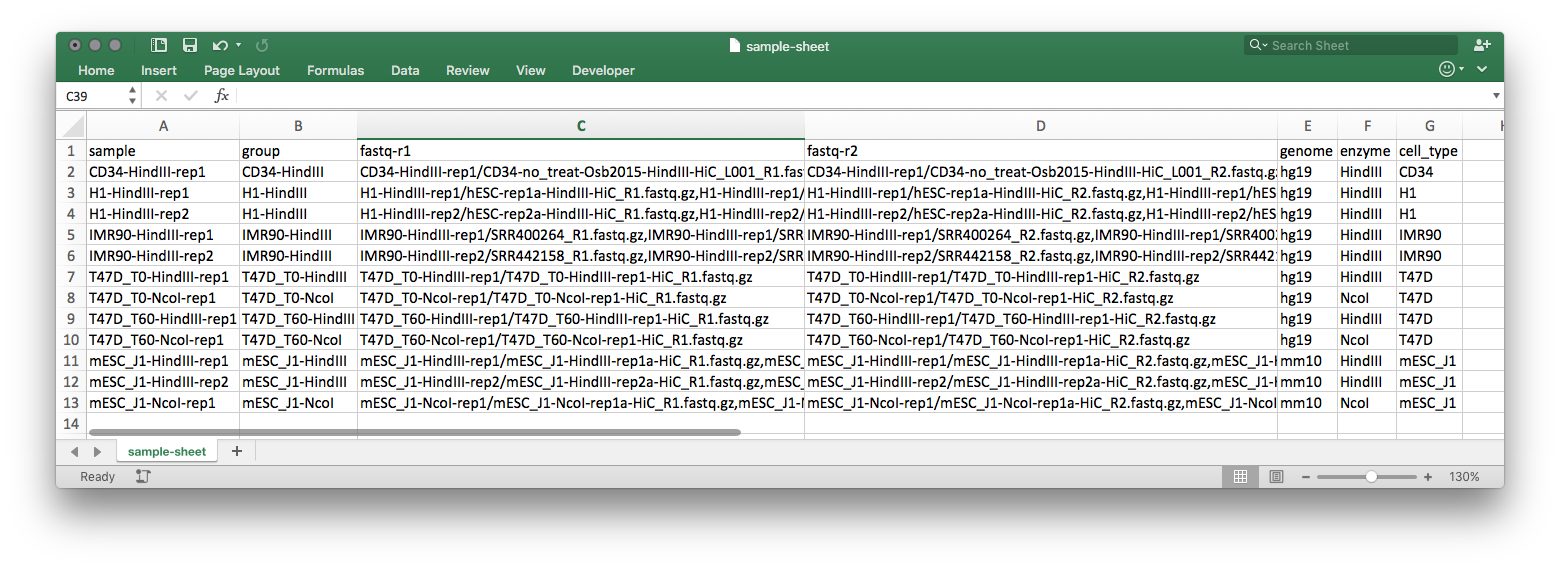
\includegraphics[width=\textwidth,height=\textheight,keepaspectratio]{figure/sample_sheet_screenshot.png}
    \caption{Example sample sheet}
    \label{fig:label}
\end{figure}

%~~~~~~~~~~~~~~~~~~~%
\subsection{Running the Pipeline}\label{Intro:pipeline-execute}
 
After navigating to the parent directory of the analysis project, run the pipeline with:
\begin{lstlisting}
./code.main/pipeline-execute PROJECT-NAME E-MAIL
\end{lstlisting}

\clearpage